\documentclass[aspectratio=169]{beamer}
\usepackage{lmodern}
%\usetheme{Madrid}
%\usecolortheme{giantoak}
\newcommand*\oldmacro{}
\let\oldmacro\insertshorttitle
\renewcommand*\insertshorttitle{\oldmacro\hfill\insertframenumber\,/\,\inserttotalframenumber}
\usepackage[framemethod=tikz]{mdframed}

%\usepackage{beamerthemesplit}
\usepackage{textpos}
\usepackage{pgf}
\usepackage{ulem}
%\logo{\pgfputat{\pgfxy(0,-.4)}{\pgfbox[right,base]{\includegraphics[height=1.0cm]{logo.jpg}}}}
%\newcommand{\nologo}{\setbeamertemplate{logo}{}}
\usepackage{booktabs}
\usepackage{graphicx}
\theoremstyle{principle}
\newtheorem*{principle}{Design Principle}


\titlegraphic{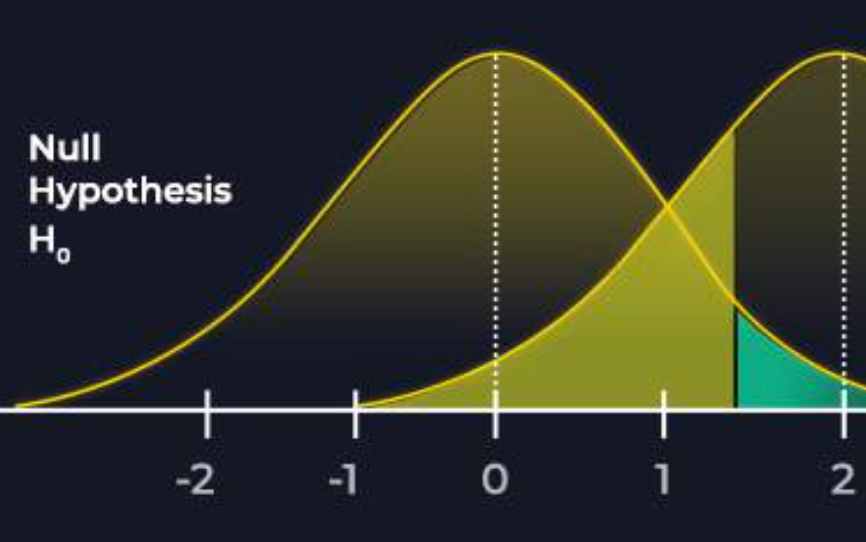
\includegraphics[width=1.0\paperwidth]{distros.png}}

\title{Amendments}
%\author[Jeremy Kedziora]{Wind Data Science Team\\
%\small{Uptake}}
\date{}

\begin{document}

%{
%%\nologo
%\begin{frame}
%    \maketitle
%\end{frame}
%}
%pages 1-7, 8-9, 14-15.


{
%  \usebackgroundtemplate{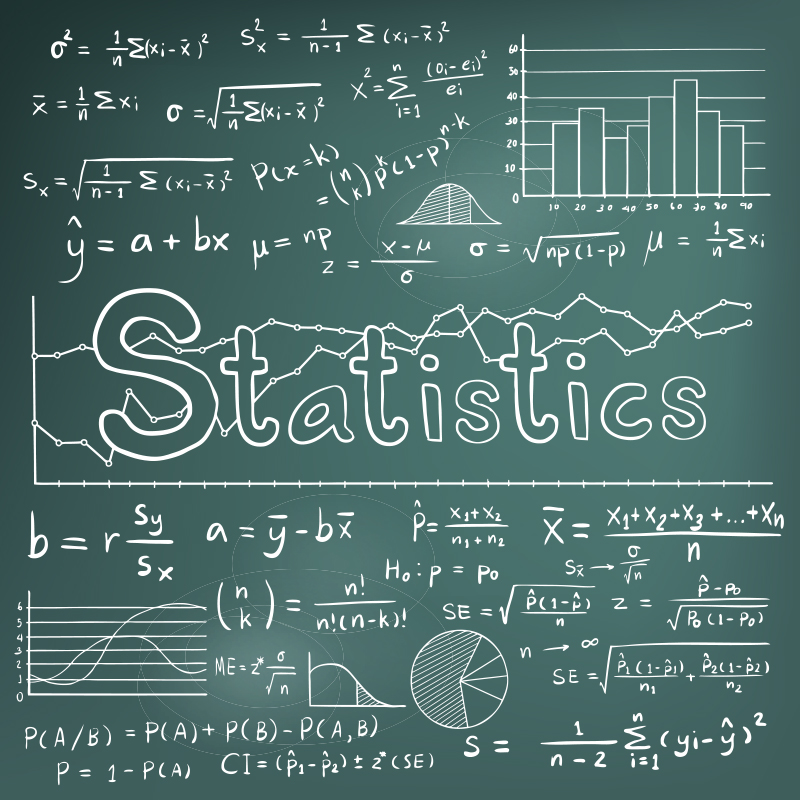
\includegraphics[width=1.0\paperwidth]{statistics-review.jpg}}
  \usebackgroundtemplate{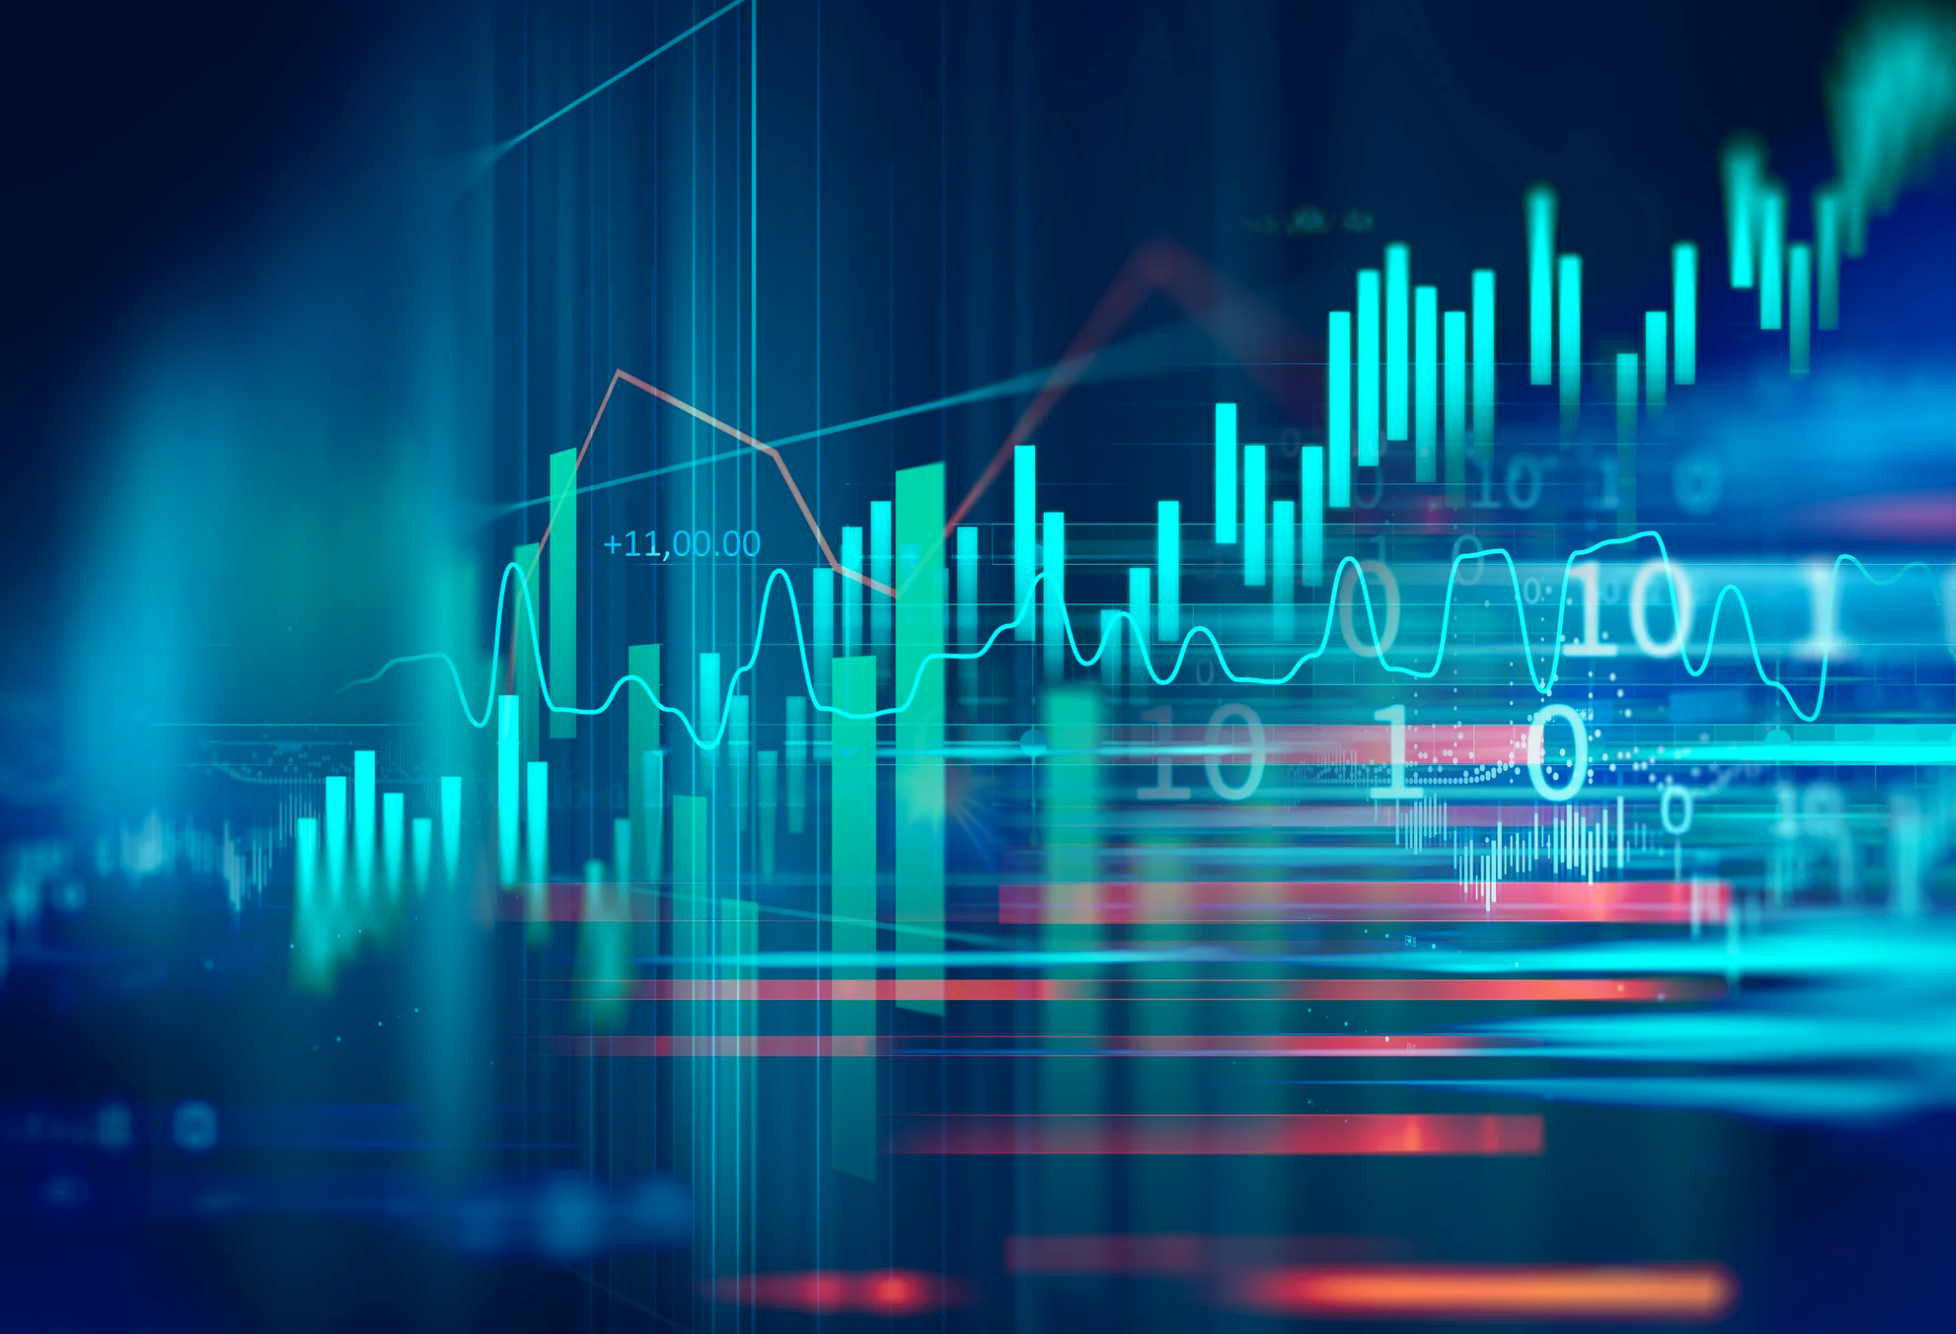
\includegraphics[scale=0.5]{pretty_data.png}}
  \begin{frame}[plain]
  
\begin{mdframed}[tikzsetting={draw=white,fill=white,fill opacity=0.6,draw opacity=0.4,
               line width=0pt},backgroundcolor=none,leftmargin=20,
               rightmargin=20,innertopmargin=4pt]
\begin{center}
\Huge \textbf{Linear Regression}
\end{center}
\end{mdframed}

  \end{frame}
}

%most reliant on human cognition
%limited only by cognition
%hypothesis generating scheme often functioning as a gateway into more statistical analysis

%%@@@@@@@@@@@@@@@@@@@@@@@@@@@@@@@@@@@@@@@@@@@@@@@@@
%\begin{frame}
%\frametitle{Napoleon's Progress}
%\begin{center}
%
\includegraphics[scale=0.4]{experiment.png}
%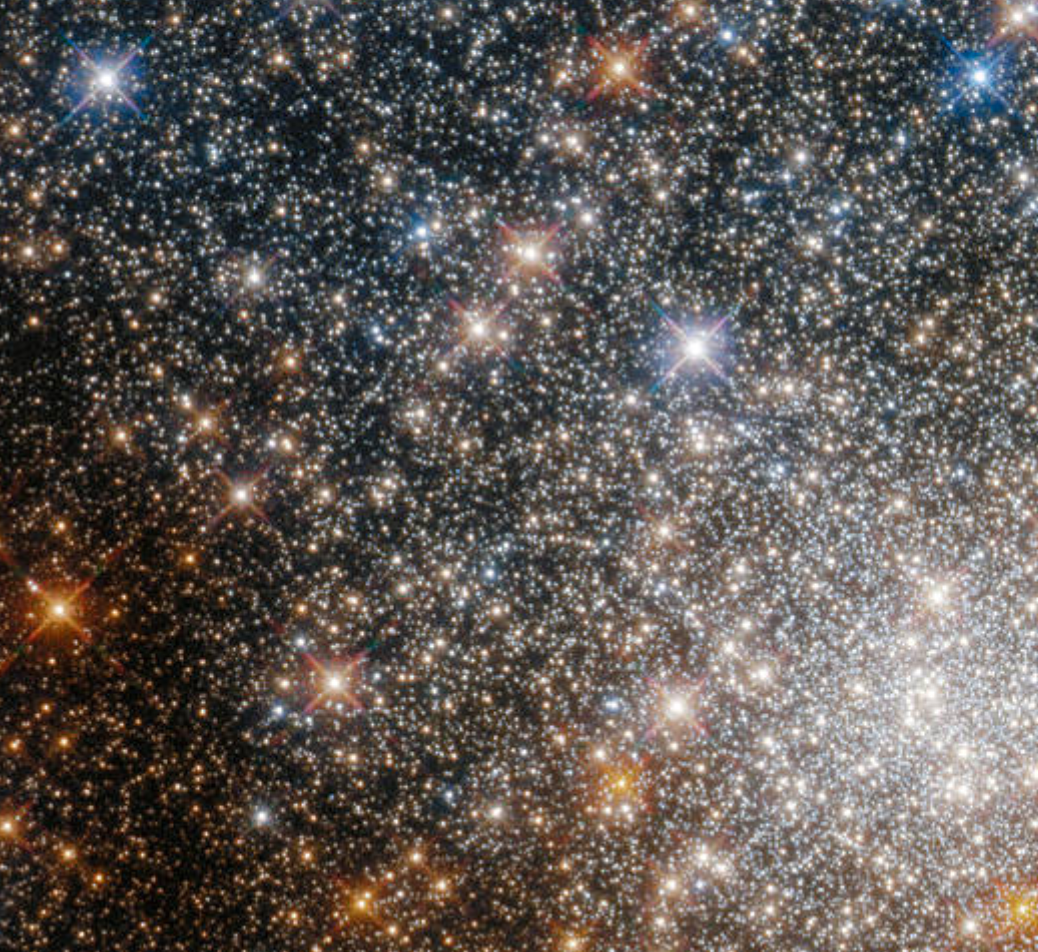
\includegraphics[scale=0.35]{stars.png}
%\end{center}
%
%\end{frame}

%@@@@@@@@@@@@@@@@@@@@@@@@@@@@@@@@@@@@@@@@@@@@@@@@@
\begin{frame}
\frametitle{Today:}

\begin{itemize}
\item Understand linear regression as a statistical model;
\bigskip
\bigskip
\bigskip

\item Introduce an example dataset;
\bigskip
\bigskip
\bigskip

\item Build the ability to interpret linear regression results.

\end{itemize}

\end{frame}

%@@@@@@@@@@@@@@@@@@@@@@@@@@@@@@@@@@@@@@@@@@@@@@@@@
\begin{frame}
\frametitle{What is linear regression?}

\begin{itemize}
\item \textbf{Linear regression} is a method that answers three questions simultaneously:
\begin{enumerate}
\item What is the effect of one variable $x$ upon another variable $y$?
\item How sure are we that $x$ affects $y$?
\item Do the answers to the first two questions depend on other independent variables?
\end{enumerate}
\bigskip
\bigskip

\item Typically used to model a dependent variable that is \textbf{continuous} (so interval or ratio data) and \textbf{unbounded} (so has no theoretical max or min);
\bigskip
\bigskip

\item The essence of the linear regression model is:
\begin{align*}
y = \beta_0 + \beta_1x + \varepsilon
\end{align*}

\end{itemize}

\end{frame}

%@@@@@@@@@@@@@@@@@@@@@@@@@@@@@@@@@@@@@@@@@@@@@@@@@
\begin{frame}
\frametitle{What is linear regression?}

\begin{itemize}
\item \textbf{Linear regression} is a method that answers three questions simultaneously:
\begin{enumerate}
\item What is the effect of one variable $x$ upon another variable $y$?
\item How sure are we that $x$ affects $y$?
\item Do the answers to the first two questions depend on other independent variables?
\end{enumerate}
\bigskip
\bigskip

\item Typically used to model a dependent variable that is \textbf{continuous} (so interval or ratio data) and \textbf{unbounded} (so has no theoretical max or min);
\bigskip
\bigskip

\item The essence of the linear regression model is:
\begin{align*}
y = \beta_0 + \beta_1x_1 + \beta_2x_2 + \hdots + \beta_mx_m + \varepsilon
\end{align*}

\end{itemize}

\end{frame}

%@@@@@@@@@@@@@@@@@@@@@@@@@@@@@@@@@@@@@@@@@@@@@@@@@
\begin{frame}
\frametitle{What is linear regression?}
\begin{center}\huge
\begin{align*}
y = \beta_0 + \beta_1x_1 + \beta_2x_2 + \hdots + \beta_mx_m + \varepsilon
\end{align*}
\end{center}
\bigskip
\bigskip

\begin{itemize}
\item $y$ is the \textbf{dependent variable} -- this is part of the data set;
\item The $x$'s are \textbf{independent variables} that explain $y$ -- also part of the data set;
\item The $\beta$'s are called \textbf{coefficient effects} that control how the $x$'s affect $y$ -- they are \textbf{learned} from the data;
\item Finally the $\varepsilon$ is a \textbf{noise} term that models the fact that $y$ may also depend on random stuff (we don't observe this but use it to learn the $\beta$'s -- that'll be for next time).

\end{itemize}
\bigskip
\bigskip

\end{frame}

%@@@@@@@@@@@@@@@@@@@@@@@@@@@@@@@@@@@@@@@@@@@@@@@@@
\begin{frame}

\begin{center}
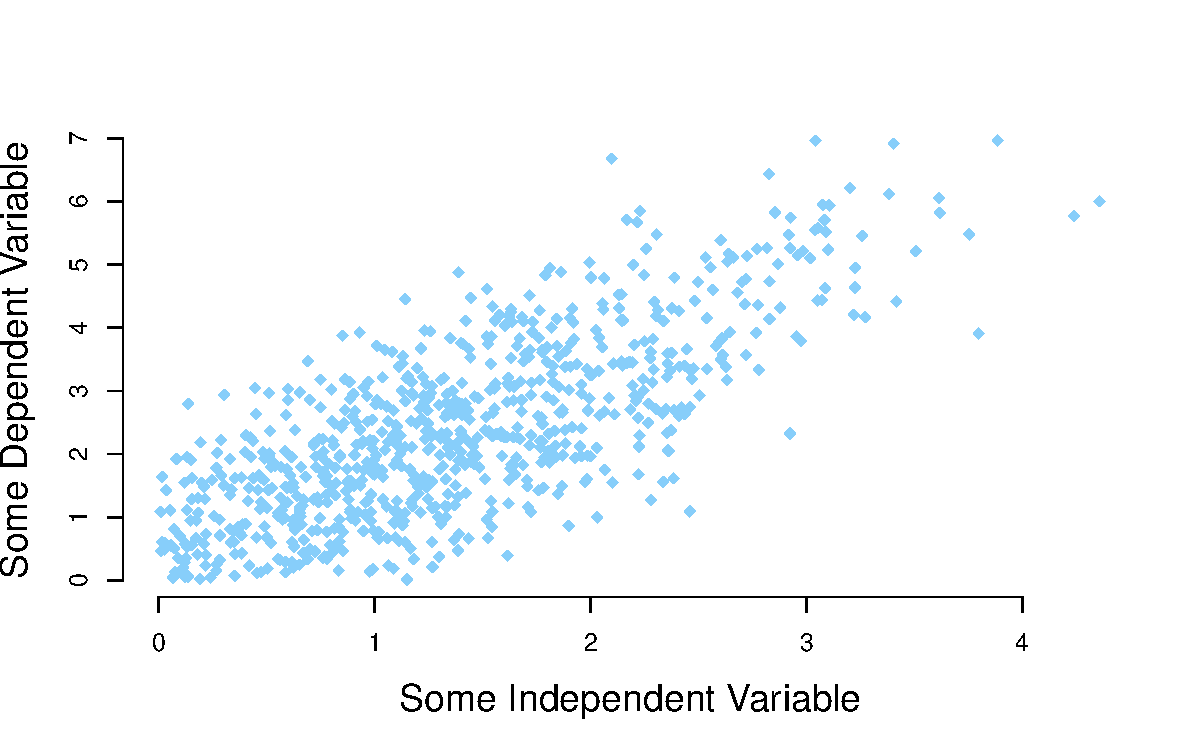
\includegraphics[scale=0.6]{point_cloud.pdf}
\end{center}

\end{frame}

%@@@@@@@@@@@@@@@@@@@@@@@@@@@@@@@@@@@@@@@@@@@@@@@@@
\begin{frame}

\begin{center}
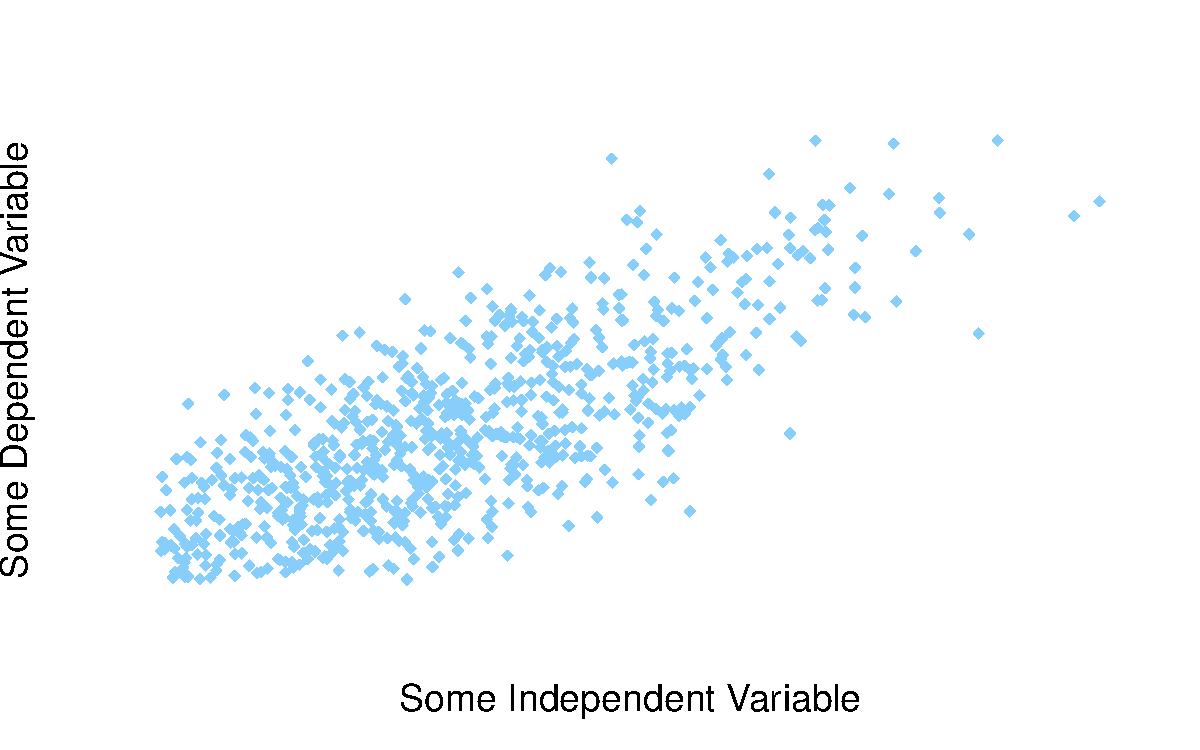
\includegraphics[scale=0.6]{point_cloud_line.pdf}
\end{center}

\end{frame}

%@@@@@@@@@@@@@@@@@@@@@@@@@@@@@@@@@@@@@@@@@@@@@@@@@
\begin{frame}
\frametitle{An Example: the US Census American Community Survey, 2012.}
\small
% latex table generated in R 4.1.1 by xtable 1.8-4 package
% Wed Oct 19 11:35:03 2022
\begin{table}[ht]
\centering
\begin{tabular}{rrlrlrllll}
  \hline
 income  & hrs & race & age & gender & cmte & lang & married & edu & disability \\ 
  \hline
 1700  &  40 & other &  35 & female  &  15 & other & yes & hs or lower & yes \\ 
 45000  &  84 & white &  27 & male  &  40 & english & yes & hs or lower & no \\ 
 8600  &  23 & white &  69 & female  &   5 & english & no & hs or lower & no \\ 
 33500  &  55 & white &  52 & male  &  20 & english & yes & hs or lower & no \\ 
 4000  &   8 & white &  67 & female  &  10 & english & yes & hs or lower & no \\ 
 19000  &  35 & white &  36 & female  &  15 & english & yes & college & no \\ 
\vdots &\vdots &\vdots &\vdots &\vdots &\vdots &\vdots &\vdots &\vdots &\vdots \\
   \hline
\end{tabular}
\end{table}
\bigskip\Large
\begin{center}
Question: do people earn more money as they get older?
\end{center}

\end{frame}

%@@@@@@@@@@@@@@@@@@@@@@@@@@@@@@@@@@@@@@@@@@@@@@@@@
\begin{frame}
\frametitle{An Example: the US Census American Community Survey, 2012.}
\small
% latex table generated in R 4.1.1 by xtable 1.8-4 package
% Wed Oct 19 11:35:03 2022
\begin{table}[ht]
\centering
\begin{tabular}{rrlrlrllll}
  \hline
 \textbf{income}  & hrs & race & \textbf{age} & gender & cmte & lang & married & edu & disability \\ 
  \hline
 1700  &  40 & other &  35 & female  &  15 & other & yes & hs or lower & yes \\ 
 45000  &  84 & white &  27 & male  &  40 & english & yes & hs or lower & no \\ 
 8600  &  23 & white &  69 & female  &   5 & english & no & hs or lower & no \\ 
 33500  &  55 & white &  52 & male  &  20 & english & yes & hs or lower & no \\ 
 4000  &   8 & white &  67 & female  &  10 & english & yes & hs or lower & no \\ 
 19000  &  35 & white &  36 & female  &  15 & english & yes & college & no \\ 
\vdots &\vdots &\vdots &\vdots &\vdots &\vdots &\vdots &\vdots &\vdots &\vdots \\
   \hline
\end{tabular}
\end{table}
\bigskip\Large
\begin{center}
Question: do people earn more money as they get older?
\end{center}

\end{frame}

%@@@@@@@@@@@@@@@@@@@@@@@@@@@@@@@@@@@@@@@@@@@@@@@@@
\begin{frame}
\frametitle{Do people earn more money as they get older?}

\begin{center}
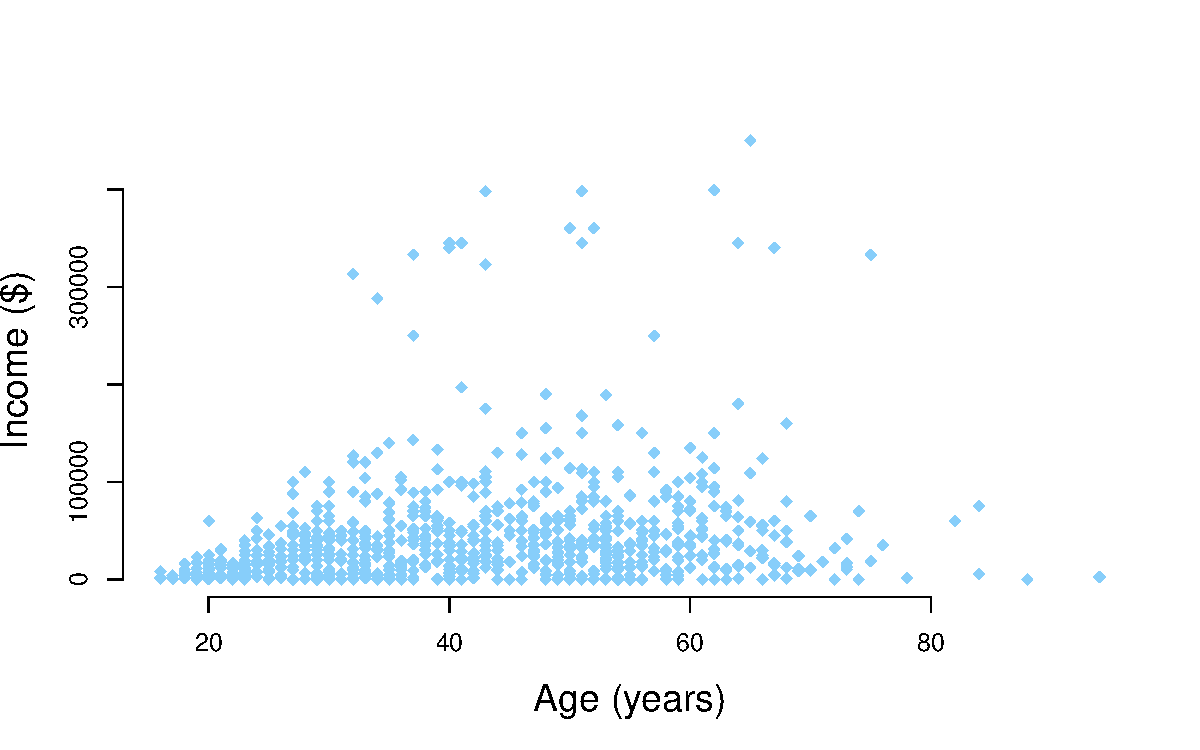
\includegraphics[scale=0.6]{income_v_age.pdf}
\end{center}

\end{frame}


%\item Remember the \textbf{binomial distribution} that models the probability of $k$ successes in $n$ trials given that each trial has probability of success $\pi$?
%\bigskip
%\bigskip
%
%\item Let's use this to compute the null distribution (the distribution over the number of Johnson voters in a sample of 15 given that $H_0$ is true so that $\pi = 0.5$).
%\bigskip

%%@@@@@@@@@@@@@@@@@@@@@@@@@@@@@@@@@@@@@@@@@@@@@@@@@
%\begin{frame}
%\frametitle{An IRL example: polling in 1936...}
%
%\begin{columns}
%\begin{column}{0.5\textwidth}
%
%\begin{itemize}
%\item Blar;
%
%\item Blar;
%
%\item Blar;
%
%\end{itemize}
%
%\end{column}
%\begin{column}{0.5\textwidth}
%\begin{center}
%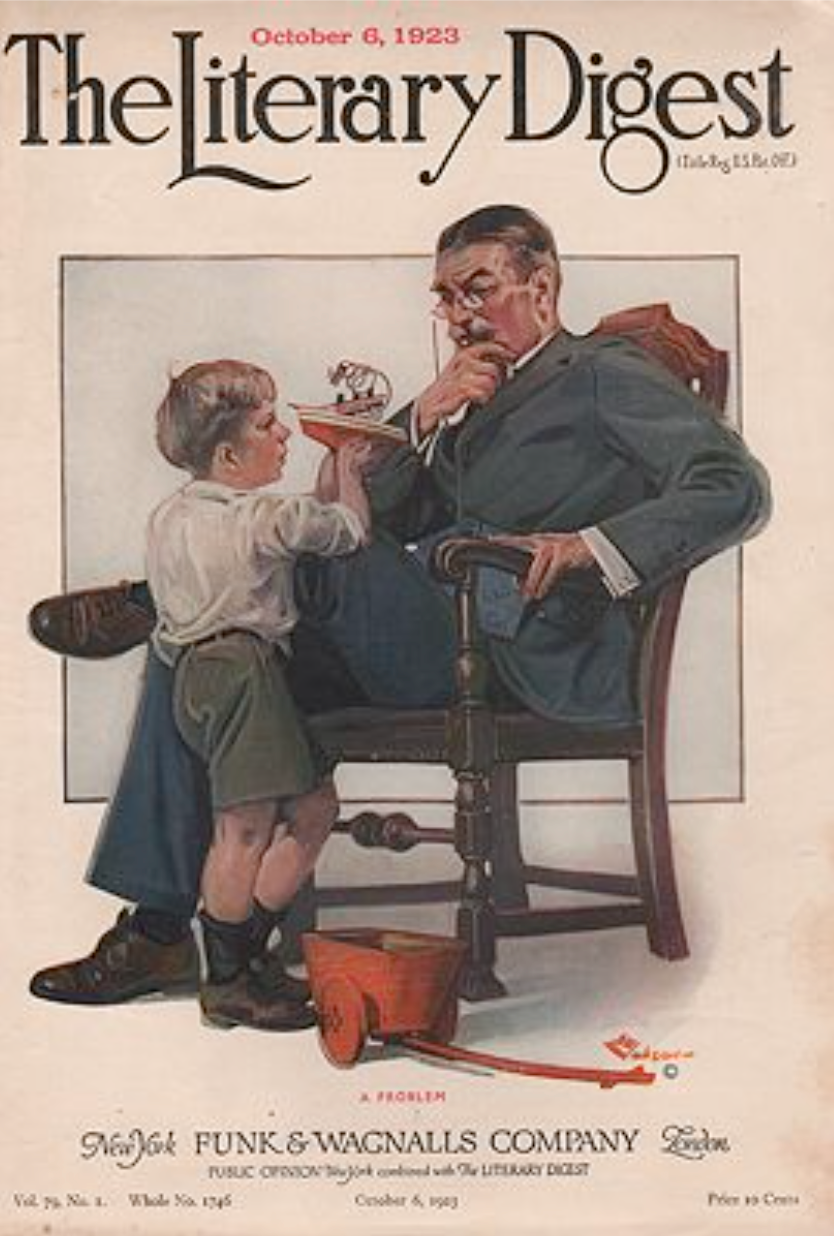
\includegraphics[scale=0.3]{LD.png}
%\end{center}
%\end{column}
%\end{columns}
%
%\end{frame}

%@@@@@@@@@@@@@@@@@@@@@@@@@@@@@@@@@@@@@@@@@@@@@@@@@
\begin{frame}
\frametitle{Do people earn more money as they get older?}

\begin{itemize}
\item Let's answer this question by building a simple regression model;
\begin{itemize}
\item The dependent variable $y$ will be \textbf{income} from the 2012 US Census American Community Survey;
\item The independent variable $x$ will be \textbf{age} from the 2012 US Census American Community Survey;
\item We will add an intercept or constant;
\end{itemize}
\bigskip
\bigskip

\item This leads to the regression equation:
\begin{align*}
income = \beta_{0} + \beta_{age}*age + \varepsilon;
\end{align*}

\item When we run the linear regression we will learn $\beta_{0}$ and $\beta_{age}$.

\end{itemize}

\end{frame}

%@@@@@@@@@@@@@@@@@@@@@@@@@@@@@@@@@@@@@@@@@@@@@@@@@
\begin{frame}
\frametitle{Do people earn more money as they get older -- results!}
\vspace{21.5mm}
\begin{center}
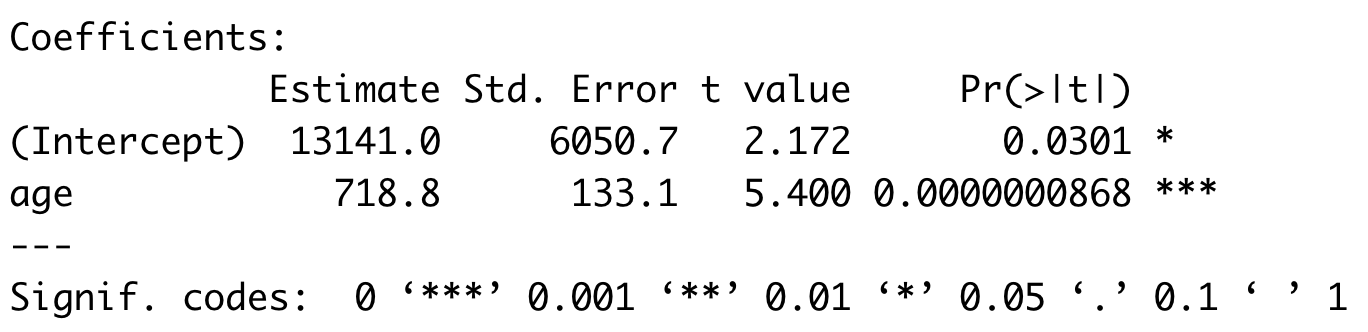
\includegraphics[scale=0.5]{income_v_age_regression_coef.png}
\end{center}

\end{frame}

%@@@@@@@@@@@@@@@@@@@@@@@@@@@@@@@@@@@@@@@@@@@@@@@@@
\begin{frame}
\frametitle{Do people earn more money as they get older -- results!}

\begin{center}
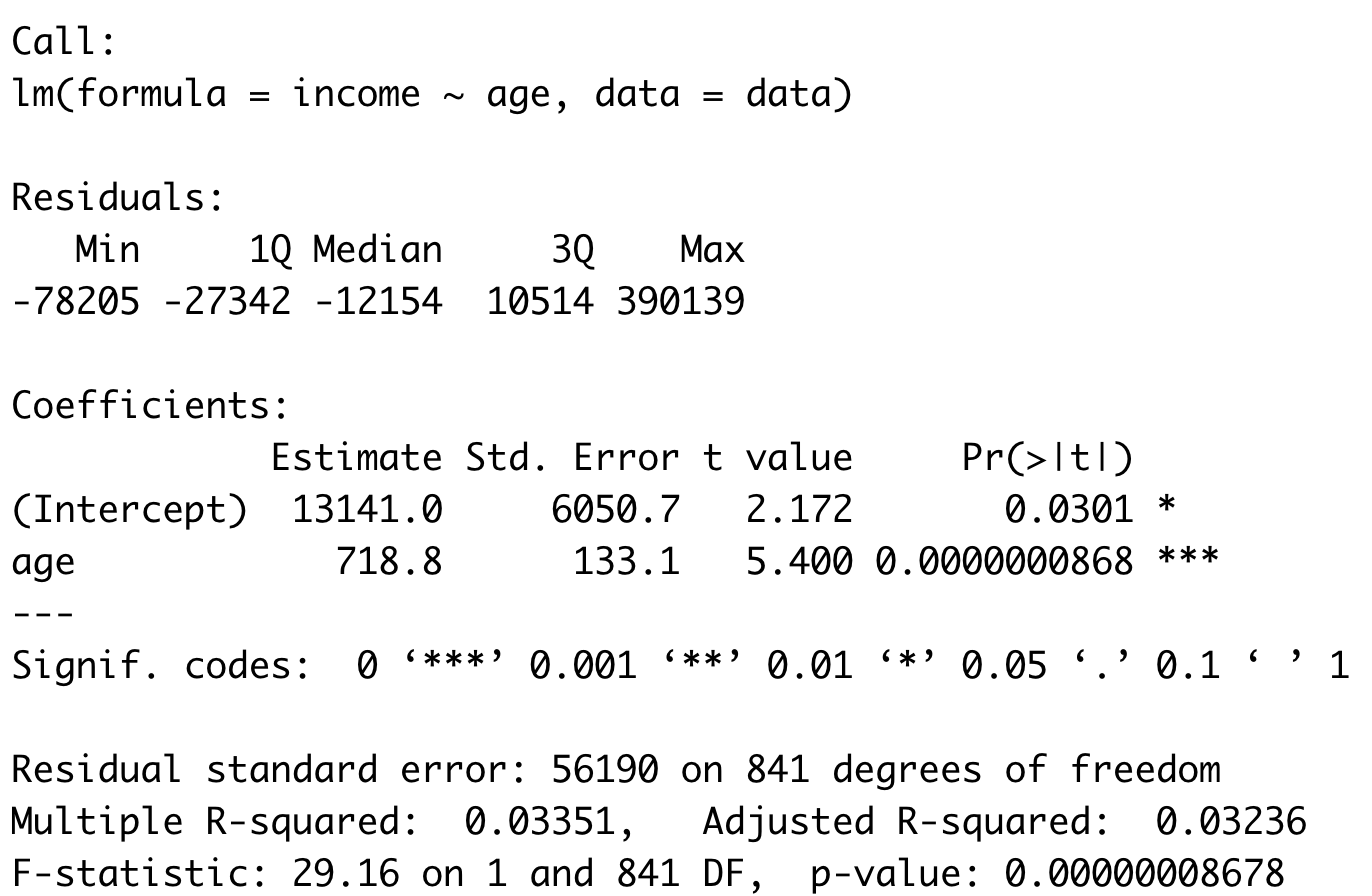
\includegraphics[scale=0.5]{income_v_age_regression.png}
\end{center}

\end{frame}

%@@@@@@@@@@@@@@@@@@@@@@@@@@@@@@@@@@@@@@@@@@@@@@@@@
\begin{frame}
\frametitle{An Example: the US Census American Community Survey, 2012.}
\small
% latex table generated in R 4.1.1 by xtable 1.8-4 package
% Wed Oct 19 11:35:03 2022
\begin{table}[ht]
\centering
\begin{tabular}{rrlrlrllll}
  \hline
\textbf{income}  & \textbf{hrs} & race & age & \textbf{gender} & \textbf{cmte} & lang & married & \textbf{edu} & disability \\ 
  \hline
 1700  &  40 & other &  35 & female  &  15 & other & yes & hs or lower & yes \\ 
 45000  &  84 & white &  27 & male  &  40 & english & yes & hs or lower & no \\ 
 8600  &  23 & white &  69 & female  &   5 & english & no & hs or lower & no \\ 
 33500  &  55 & white &  52 & male  &  20 & english & yes & hs or lower & no \\ 
 4000  &   8 & white &  67 & female  &  10 & english & yes & hs or lower & no \\ 
 19000  &  35 & white &  36 & female  &  15 & english & yes & college & no \\ 
\vdots &\vdots &\vdots &\vdots &\vdots &\vdots &\vdots &\vdots &\vdots &\vdots \\
   \hline
\end{tabular}
\end{table}
\bigskip\Large
\begin{center}
Question: do people earn more money as they get older?
\end{center}

\end{frame}

%@@@@@@@@@@@@@@@@@@@@@@@@@@@@@@@@@@@@@@@@@@@@@@@@@
\begin{frame}
\frametitle{Do people earn more money as they get older -- results!}

\begin{center}
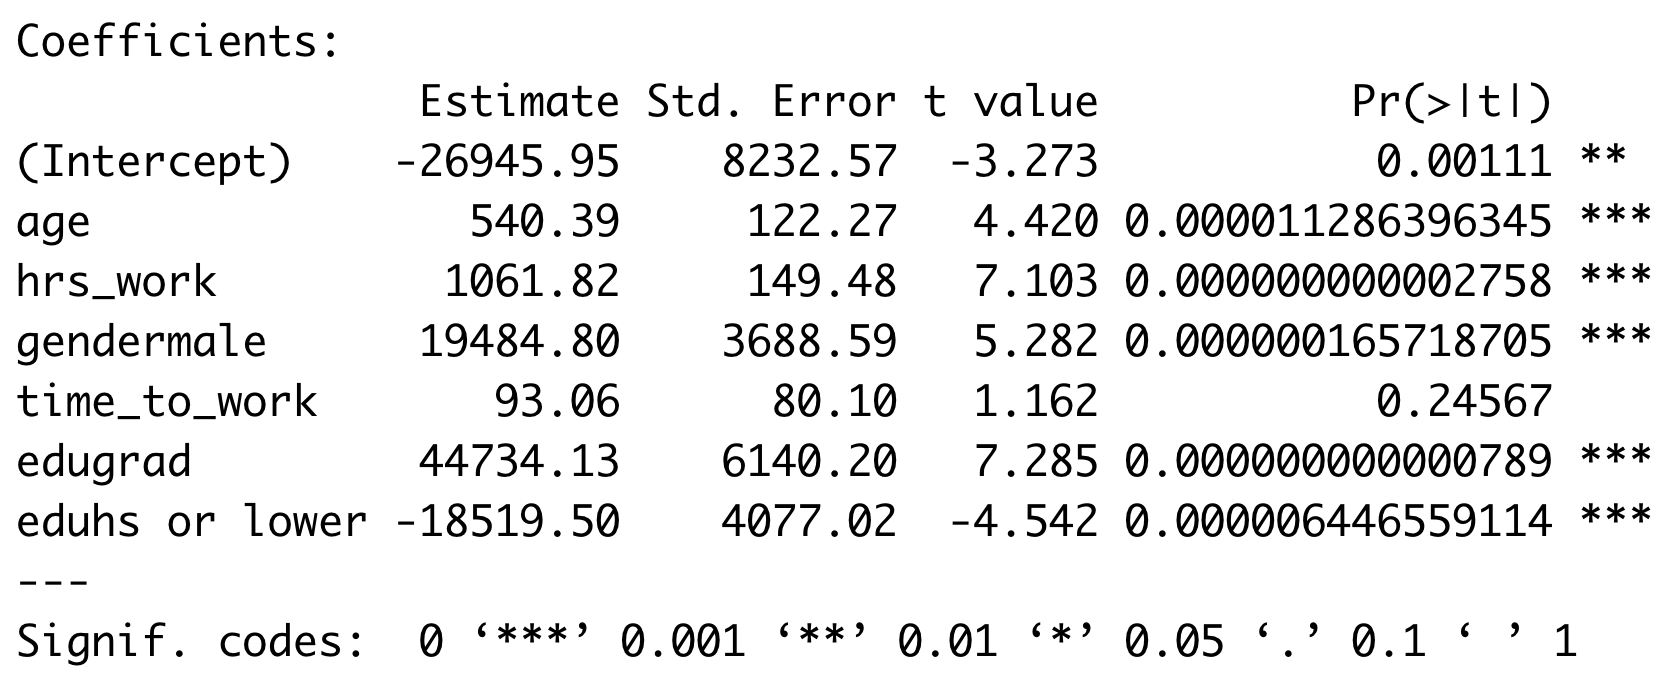
\includegraphics[scale=0.4]{income_v_age_full.png}
\end{center}

\end{frame}

%@@@@@@@@@@@@@@@@@@@@@@@@@@@@@@@@@@@@@@@@@@@@@@@@@
\begin{frame}
\frametitle{How does linear regression work?}
\begin{center}
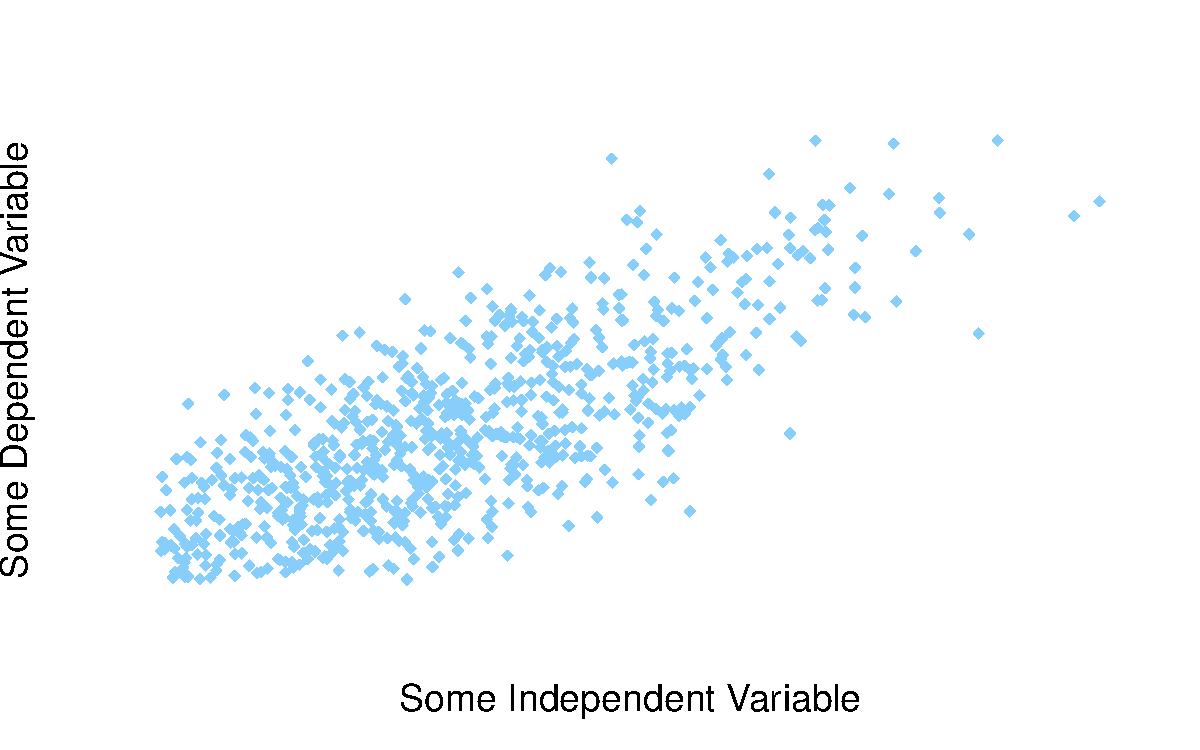
\includegraphics[scale=0.6]{point_cloud_line.pdf}
\end{center}

\end{frame}

%@@@@@@@@@@@@@@@@@@@@@@@@@@@@@@@@@@@@@@@@@@@@@@@@@
\begin{frame}
\frametitle{How does linear regression work?}
\begin{center}
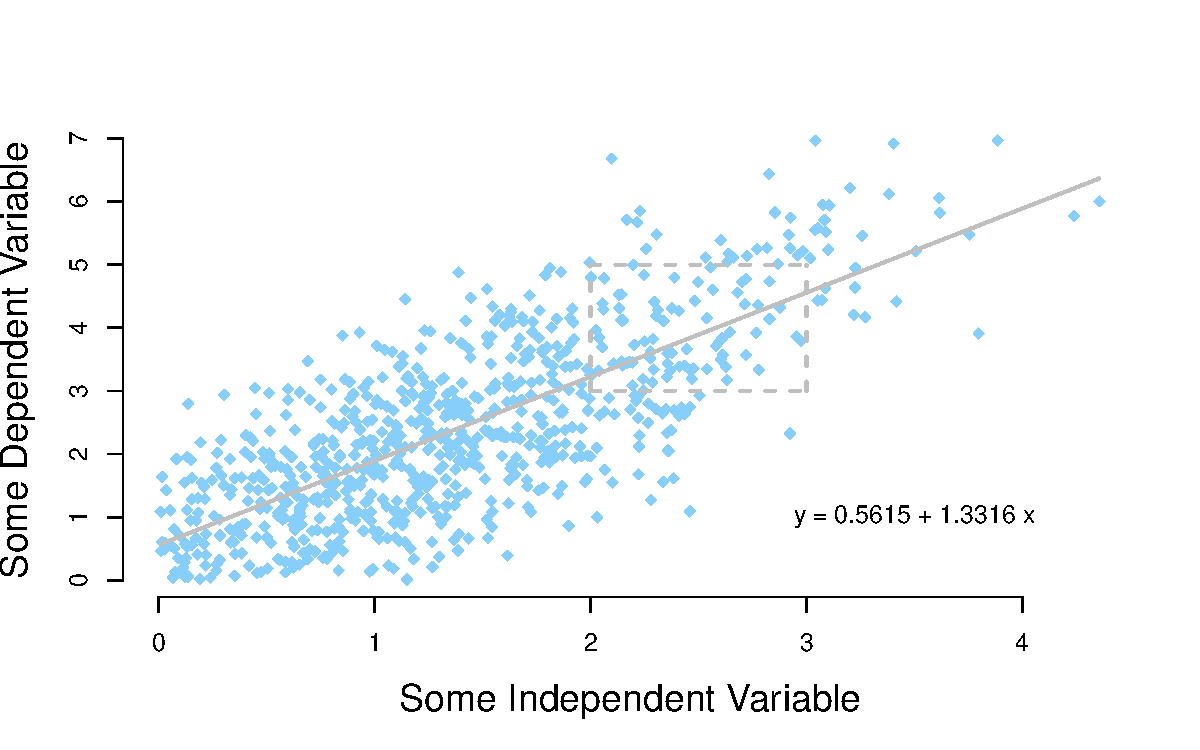
\includegraphics[scale=0.6]{point_cloud_line_box.pdf}
\end{center}

\end{frame}

%@@@@@@@@@@@@@@@@@@@@@@@@@@@@@@@@@@@@@@@@@@@@@@@@@
\begin{frame}
\frametitle{How does linear regression work?}
\begin{center}
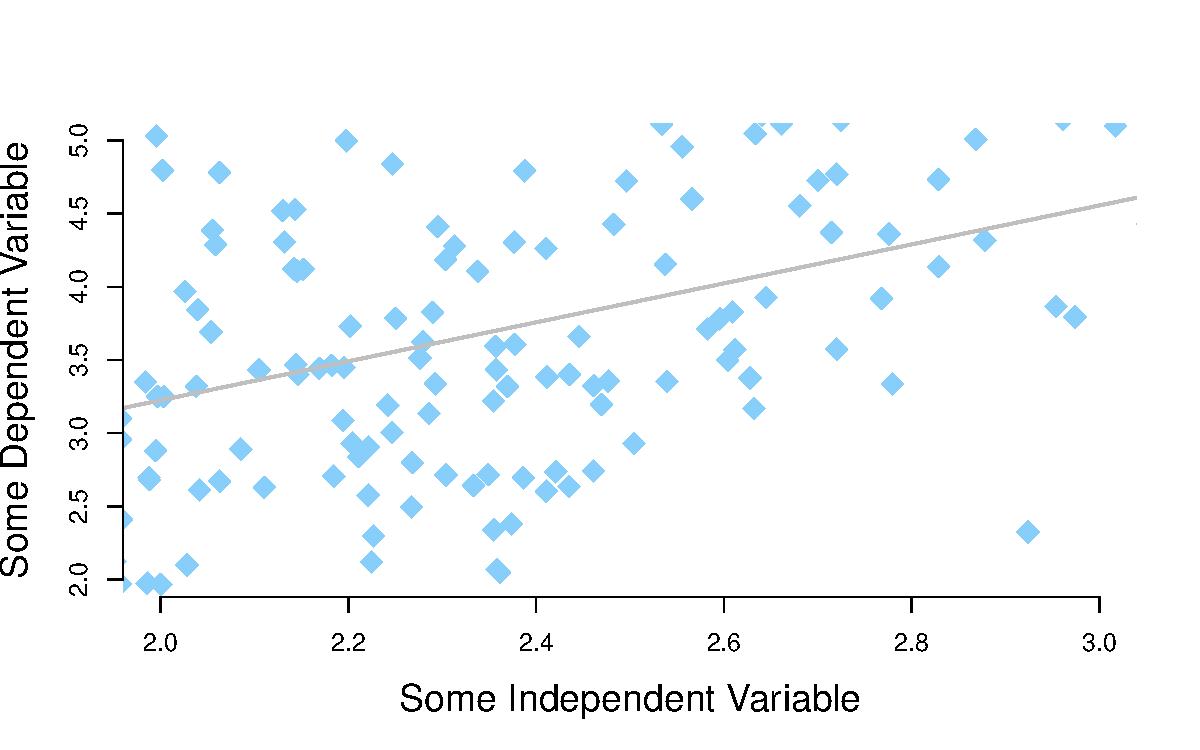
\includegraphics[scale=0.6]{point_cloud_line_zoomed.pdf}
\end{center}

\end{frame}

%@@@@@@@@@@@@@@@@@@@@@@@@@@@@@@@@@@@@@@@@@@@@@@@@@
\begin{frame}
\frametitle{How does linear regression work?}
\begin{center}
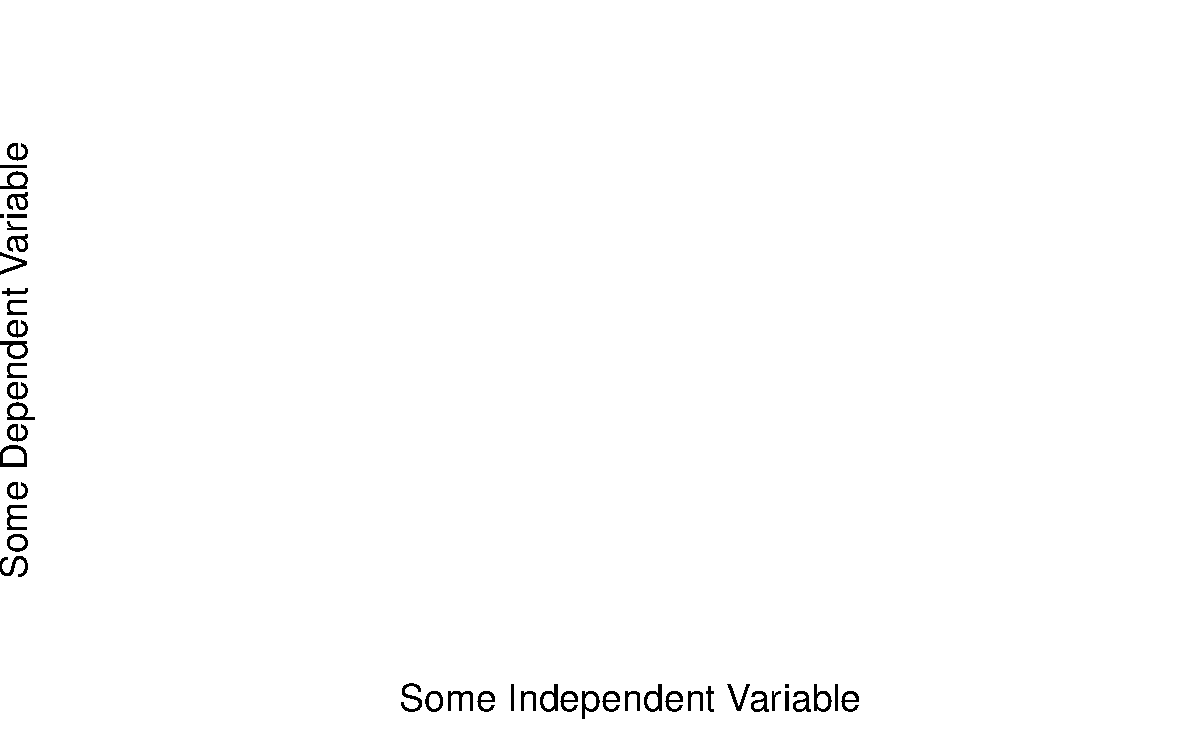
\includegraphics[scale=0.6]{point_cloud_line_zoomed_residual.pdf}
\end{center}

\end{frame}

%@@@@@@@@@@@@@@@@@@@@@@@@@@@@@@@@@@@@@@@@@@@@@@@@@
\begin{frame}
\frametitle{How does linear regression work?}
\begin{center}
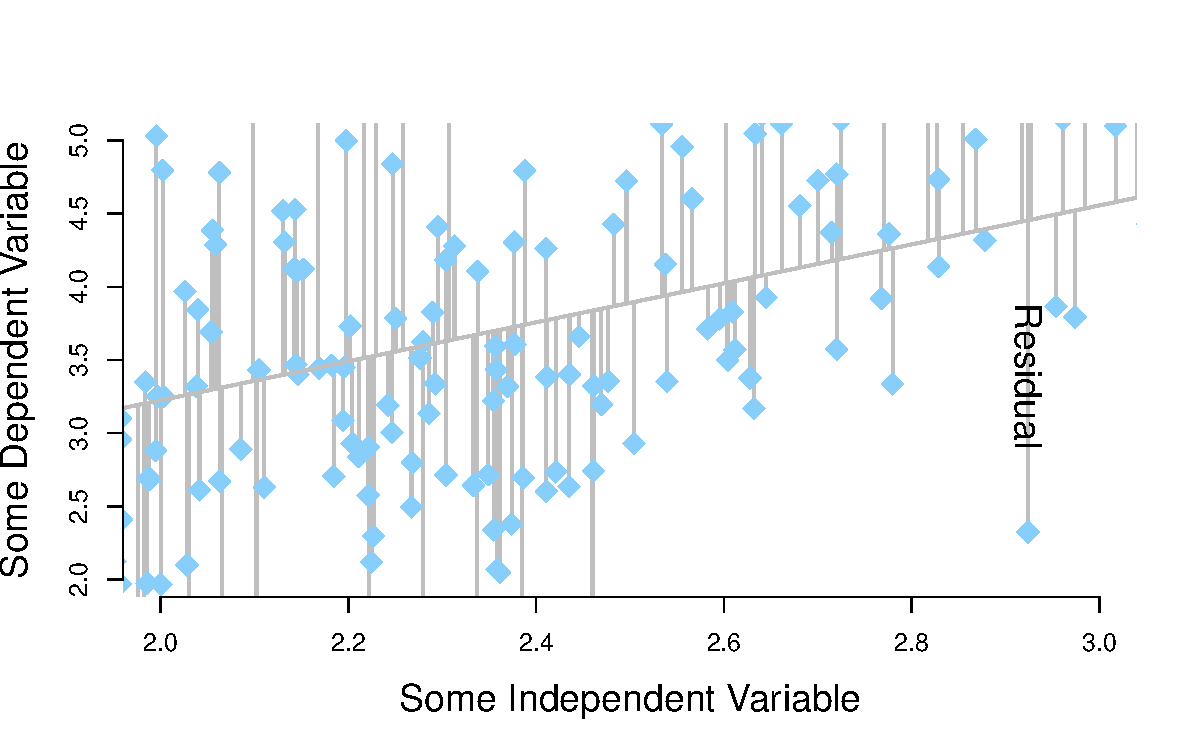
\includegraphics[scale=0.6]{point_cloud_line_zoomed_residuals.pdf}
\end{center}

\end{frame}

%@@@@@@@@@@@@@@@@@@@@@@@@@@@@@@@@@@@@@@@@@@@@@@@@@
\begin{frame}
\frametitle{How does linear regression work?}

\begin{itemize}
\item Linear regression finds the `line of best fit.'  What does this mean?  It means finding the `best' $\beta$s;
\bigskip

\item Linear regression finds the best $\beta$s by minimizing the sum of residuals;
\bigskip

\item How?
\begin{enumerate}
\item Take the observed dependent variable for an observation...
\item[]\color{white} Given some $\beta$s and the independent variables create the prediction...
\item[]\color{white} Take the difference between the two...
\item[]\color{white} Square the difference...
\item[]\color{white} Add it up for all the observations in the data...
\item[]\color{white} Choose the $\beta$s that make this as small as possible...
\end{enumerate}
\begin{align*}
\color{white}\min_{\beta_0,\beta_1}\sum_i(\color{black}y_i\color{white} - (\beta_0 + \beta_1 x_i))^2
\end{align*}
\end{itemize}

\end{frame}

%@@@@@@@@@@@@@@@@@@@@@@@@@@@@@@@@@@@@@@@@@@@@@@@@@
\begin{frame}
\frametitle{How does linear regression work?}

\begin{itemize}
\item Linear regression finds the `line of best fit.'  What does this mean?  It means finding the `best' $\beta$s;
\bigskip

\item Linear regression finds the best $\beta$s by minimizing the sum of residuals;
\bigskip

\item How?
\begin{enumerate}
\item Take the observed dependent variable for an observation...
\item Given some $\beta$s and the independent variables create a prediction...
\item[]\color{white} Take the difference between the two...
\item[]\color{white} Square the difference...
\item[]\color{white} Add it up for all the observations in the data...
\item[]\color{white} Choose the $\beta$s that make this as small as possible...
\end{enumerate}
\begin{align*}
\color{white}\min_{\beta_0,\beta_1}\sum_i(\color{black}y_i\color{white} - (\color{black}\beta_0 + \beta_1 x_i\color{white}))^2
\end{align*}
\end{itemize}

\end{frame}

%@@@@@@@@@@@@@@@@@@@@@@@@@@@@@@@@@@@@@@@@@@@@@@@@@
\begin{frame}
\frametitle{How does linear regression work?}

\begin{itemize}
\item Linear regression finds the `line of best fit.'  What does this mean?  It means finding the `best' $\beta$s;
\bigskip

\item Linear regression finds the best $\beta$s by minimizing the sum of residuals;
\bigskip

\item How?
\begin{enumerate}
\item Take the observed dependent variable for an observation...
\item Given some $\beta$s and the independent variables create a prediction...
\item Take the difference between the two (this is the residual)...
\item[]\color{white} Square the difference...
\item[]\color{white} Add it up for all the observations in the data...
\item[]\color{white} Choose the $\beta$s that make this as small as possible...
\end{enumerate}
\begin{align*}
\color{white}\min_{\beta_0,\beta_1}\sum_i(\color{black}y_i - (\beta_0 + \beta_1 x_i)\color{white})^2
\end{align*}
\end{itemize}

\end{frame}

%@@@@@@@@@@@@@@@@@@@@@@@@@@@@@@@@@@@@@@@@@@@@@@@@@
\begin{frame}
\frametitle{How does linear regression work?}

\begin{itemize}
\item Linear regression finds the `line of best fit.'  What does this mean?  It means finding the `best' $\beta$s;
\bigskip

\item Linear regression finds the best $\beta$s by minimizing the sum of residuals;
\bigskip

\item How?
\begin{enumerate}
\item Take the observed dependent variable for an observation...
\item Given some $\beta$s and the independent variables create a prediction...
\item Take the difference between the two (this is the residual)...
\item Square the difference...
\item[]\color{white} Add it up for all the observations in the data...
\item[]\color{white} Choose the $\beta$s that make this as small as possible...
\end{enumerate}
\begin{align*}
\color{white}\min_{\beta_0,\beta_1}\sum_i\color{black}(y_i - (\beta_0 + \beta_1 x_i))^2
\end{align*}
\end{itemize}

\end{frame}

%@@@@@@@@@@@@@@@@@@@@@@@@@@@@@@@@@@@@@@@@@@@@@@@@@
\begin{frame}
\frametitle{How does linear regression work?}

\begin{itemize}
\item Linear regression finds the `line of best fit.'  What does this mean?  It means finding the `best' $\beta$s;
\bigskip

\item Linear regression finds the best $\beta$s by minimizing the sum of residuals;
\bigskip

\item How?
\begin{enumerate}
\item Take the observed dependent variable for an observation...
\item Given some $\beta$s and the independent variables create a prediction...
\item Take the difference between the two (this is the residual)...
\item Square the difference...
\item Add it up for all the observations in the data...
\item[]\color{white} Choose the $\beta$s that make this as small as possible...
\end{enumerate}
\begin{align*}
\color{white}\min_{\beta_0,\beta_1}\color{black}\sum_i(y_i - (\beta_0 + \beta_1 x_i))^2
\end{align*}
\end{itemize}

\end{frame}

%@@@@@@@@@@@@@@@@@@@@@@@@@@@@@@@@@@@@@@@@@@@@@@@@@
\begin{frame}
\frametitle{How does linear regression work?}

\begin{itemize}
\item Linear regression finds the `line of best fit.'  What does this mean?  It means finding the `best' $\beta$s;
\bigskip

\item Linear regression finds the best $\beta$s by minimizing the sum of residuals;
\bigskip

\item How?
\begin{enumerate}
\item Take the observed dependent variable for an observation...
\item Given some $\beta$s and the independent variables create a prediction...
\item Take the difference between the two (this is the residual)...
\item Square the difference...
\item Add it up for all the observations in the data...
\item Choose the $\beta$s that make this as small as possible...
\end{enumerate}
\begin{align*}
\min_{\beta_0,\beta_1}\color{black}\sum_i(y_i - (\beta_0 + \beta_1 x_i))^2.
\end{align*}
\end{itemize}

\end{frame}

%@@@@@@@@@@@@@@@@@@@@@@@@@@@@@@@@@@@@@@@@@@@@@@@@@
\begin{frame}
\frametitle{Assumptions of Linear Regression}

\begin{enumerate}
\item Dependent variable is a \textbf{linear} function of independent variables plus noise;
\begin{align*}
y = \beta_0 + \beta_1x_1 + \beta_2x_2 + \hdots + \beta_mx_m + \varepsilon\\
\end{align*}

\item Independent variables have \textbf{no measurement error};
\bigskip
\bigskip

\item Independent variables are not related to each other -- \textbf{no multicollinearity};
\bigskip
\bigskip

\item Noise term is a random variable following the \textbf{normal distribution}.

\end{enumerate}

\end{frame}

%@@@@@@@@@@@@@@@@@@@@@@@@@@@@@@@@@@@@@@@@@@@@@@@@@
\begin{frame}
\frametitle{Why do we use Linear Regression?}

\begin{itemize}
\item Theorem (Gauss-Markov) When the assumptions of linear regression are met then it is the Best Linear Unbiased Estimator of the relationship between the dependent and independent variables;
\bigskip
\bigskip

\item `Unbiased' means that it will give you the correct $\beta$s on average;
\bigskip
\bigskip

\item `Best' means that it will give you the most precise estimates of those $\beta$s possible;
\bigskip
\bigskip

\item This is usually called BLUE for short.

\end{itemize}

\end{frame}

%@@@@@@@@@@@@@@@@@@@@@@@@@@@@@@@@@@@@@@@@@@@@@@@@@
\begin{frame}

\begin{center}
\Huge\textbf{Why should we care?}\\
\bigskip
\bigskip
\large Linear regression combines hypothesis testing and machine learning, and should be a first modeling stop for interval or ratio data.\\
\end{center}

\end{frame}



\end{document}






